\section*{\hfil Parte I\hfil}
\section{Questões e Respostas}
\subsection{Questão 1 - Topologia Core}
De acordo com as instruções presentes no enunciado, apresentamos de seguida 
a topologia construída, tendo em conta a alteração do tempo de propagação para
10 ms:

\paragraph{}
\begin{figure}[H]
\centering
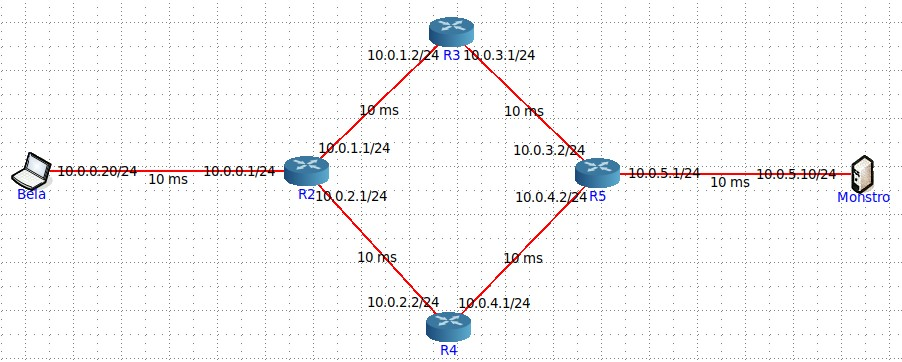
\includegraphics[width=500pt]{images/ParteI/Questao1/questao1-topologia.jpg}
\caption{Topologia (Questão 1).} \label{topologia}
\end{figure}


\paragraph{}
\subsubsection{Active o \textit{wireshark} ou o \textit{tcpdump} no \textit{host} Bela. Numa \textit{shell} de Bela execute o comando \textit{traceroute -I} para o endereço IP do Monstro}

\begin{figure}[H]
\centering
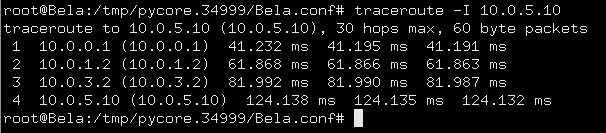
\includegraphics[width=400pt]{images/ParteI/Questao1/questao1-a.jpg}
\caption{Print da \textit{shell} no \textit{host} Bela.} \label{questao1-a}
\end{figure}

%
%
\subsubsection{Registe e analise o tráfego ICMP enviado pelo sistema Bela e o tráfego ICMP recebido como resposta. Comente os resultados face ao comportamento esperado.}



\begin{figure}[H]
\centering
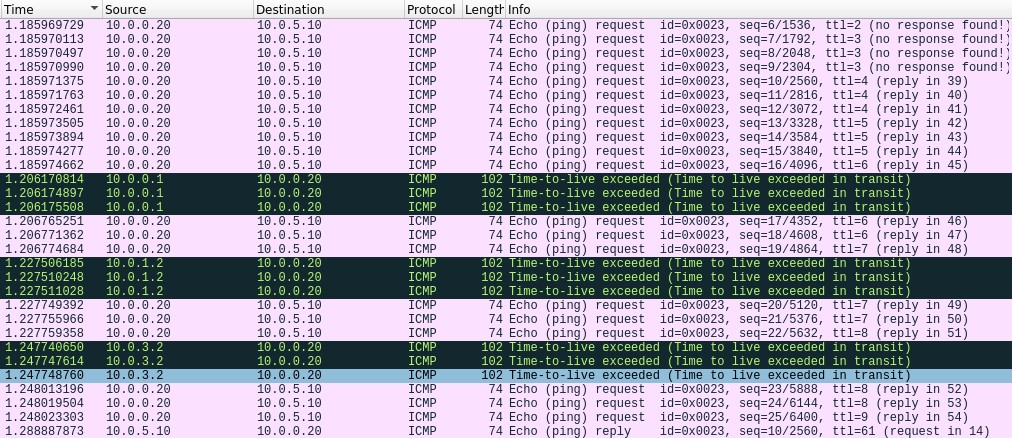
\includegraphics[width=\linewidth]{images/ParteI/Questao1/questao1-wireshark.jpg}
\caption{Tráfego ICMP enviado e recebido pelo \textit{host} Bela.} \label{1-wireshark}
\end{figure}

    O comando \textit{traceroute} envia, através do \textit{host}, vários datagramas ICMP variando o valor de TTL (\textit{Time To Live}) para assim obter a rota desde a origem até ao IP destino (especificado no comando \textit{traceroute}). A variável TTL indica o número de saltos que o datagrama pode fazer dentro da rede antes de ser considerado inválido, sendo este valor decrementado sempre que executa um salto. O seu comportamento, de forma resumida, pode ser descrito como o envio sequencial de conjuntos de um ou mais datagramas ICMP com o mesmo TTL, iniciando este valor a 1 e incrementando a cada iteração. Um \textit{host} ao verificar que o valor do TTL de um datagrama é 0 envia como resposta uma mensagem de controlo (datagrama ICMP) com a informação de 'TTL \textit{exceeded}'. Assim, o \textit{host} que enviou os datagramas iniciais vai obtendo, ao longo das iterações, uma noção cada vez mais completa da rota até ao destino.
    
    \par No caso concreto deste exercício, podemos, através da Figura \ref{1-wireshark}, verificar o envio destes conjuntos de três datagramas ICMP logo a partir da primeira linha, começando, tal como dito, no valor TTL=1 e sendo incrementado a cada iteração.
    
    \par Apresentamos, de seguida, uma tabela com a correspondência entre os valores iniciais de TTL dos datagramas e os \textit{hosts} que os receberam quando estes atingiram o valor 0, ou seja, excederam o seu número de saltos na rede: 
    
        \begin{wrapfigure}{r}{0.25\textwidth}
        \begin{center}
        \vspace{-20pt}
            \begin{tabular}{|c|c|}
            \cline{1-2}
            TTL & Host Final  \\
            \hline \hline
             1 & 10.0.0.1 \\
             2 & 10.0.1.2 \\
             3 & 10.0.3.2 \\
            \cline{1-2}
        \end{tabular}
        \end{center}
    \end{wrapfigure}
        
    \par Como podemos verificar pela tabela, os datagramas enviados com TTL=1 ficaram inválidos no \textit{host} 10.0.0.1, os datagramas com TTL=2 no \textit{host} 10.0.1.2 e, por fim, os datagramas com TTL=3 foram invalidados pelo \textit{host} 10.0.3.2. 
    
    \par Podemos reparar que os datagramas com TTL superior a 3 não registaram nenhuma resposta de 'TTL \textit{exceeded}' uma vez que a partir desse valor os pacotes conseguem chegar a qualquer nodo da rede, inclusive o nodo objetivo (10.0.5.10).
    
\subsubsection{Qual deve ser o valor inicial mínimo do campo TTL para alcançar o servidor \textit{Monstro}? Verifique na prática que a sua resposta está correta.}
    
    \par O valor mínimo do campo TTL necessário para alcançar o servidor \textit{Monstro} será \textbf{4}, uma vez que valores inferiores a 3 (inclusive) têm resposta de tempo de vida excedido (como visto na alínea anterior). Podemos verificar isto pela não receção de datagramas ICMP por parte do \textit{host} Bela a partir dos valores de TTL superiores ou iguais a 4, ou pelo cálculo direto através da observação da topologia, onde verificamos que são necessários, no mínimo, quatro saltos para atingir o servidor.



\subsubsection{Calcule o valor médio do tempo de ida-e-volta (RTT - \textit{Round-Trip Time}) obtido no acesso ao servidor. Para melhorar a média, poderá alterar o número pacotes de prova com a opção -q.}

    \begin{figure}[H]
        \centering
        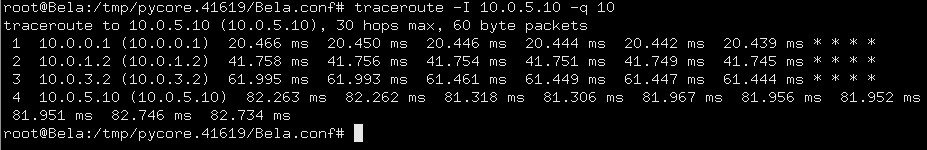
\includegraphics[width=500pt]{images/ParteI/Questao1/questao1-d.jpg}
        \caption{Aplicação do comando 'traceroute -I 10.0.5.10 -q 10'.} \label{tracerouteMedia}
    \end{figure}
    
    \par De acordo com o resultado do comando pedido, retiramos os valores atingidos no acesso ao servidor \textit{Monstro} a partir da linha numerada com o valor 4. Assim, calculamos a média destes mesmos valores, tendo obtido o seguinte resultado:

    \begin{align*}  
    \frac{82.263+82.262+81.318+81.306+81.967+81.956+81.952+81.951+82.746+82.734}{10} = 81.946 ms  
    \end{align*}  
    


\subsubsection{O valor médio do atraso num sentido (One-Way Delay) poderia ser calculado com precisão dividindo o RTT por dois? O que torna difícil o cálculo desta métrica?}
    
    O cálculo torna-se difícil devido às exigências de sincronização, uma vez que \textit{delay} é uma métrica que exige sincronização de relógios. \textit{One-Way Delay}, tal como o nome indica, só funciona num sentido, mas precisa de ter acesso a algumas informações para poder ser calculado, nomeadamente o registo de quando o pacote foi enviado (\textit{timestamp}). Em consequência, é imperativo que os relógios estejam sincronizados, caso contrário esta informação torna-se irrelevante.
     O \textit{delay} de ida é diferente do de volta pois o percurso percorrido pode não ser idêntico, por conseguinte, o valor médio de atraso num sentido não pode ser calculado com precisão dividindo o RTT por dois.
    
    

\newpage
% -------------------------- QUESTÃO 2 ------------------------------
\subsection{Questão 2 - \textit{Traceroute}}

 \begin{figure}[H]
 \centering
 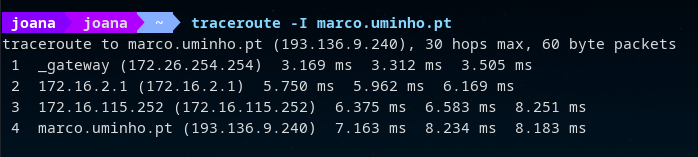
\includegraphics[width=400pt]{images/ParteI/Questao2/questao2-comando.png}
 \caption{Resultado do comando \textit{traceroute} na máquina nativa.} \label{questao2-comando}
 \end{figure}
    
 \begin{figure}[H]
 \centering
 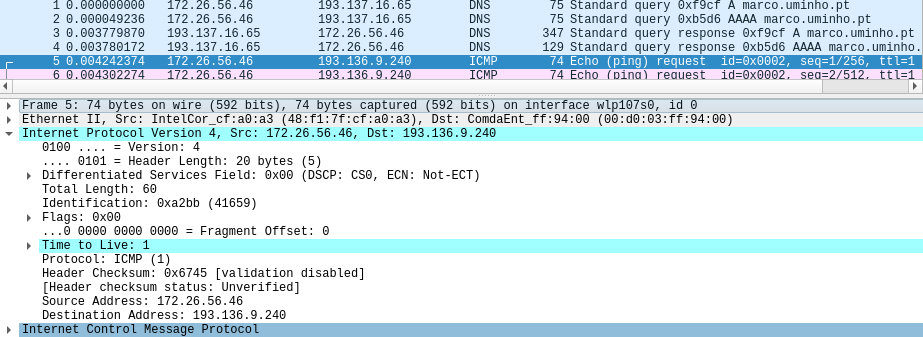
\includegraphics[width=500pt]{images/ParteI/Questao2/questao2-a)primeiroPacote.png}
 \caption{Informação da primeira mensagem ICMP enviada pela máquina.} \label{questao2-IPMaquinaNativa}
 \end{figure}
 

\subsubsection{Qual é o endereço IP da interface ativa do seu computador?}

    \par Como se pode observar na Figura \ref{questao2-IPMaquinaNativa}, na informação da mensagem ICMP enviada pela máquina nativa, no parâmetro \textit{Source Address}, a interface que foi utilizada para realizar este teste possui o endereço IP de \textbf{172.26.56.46}.


\subsubsection{Qual é o valor do campo protocolo? O que permite identificar?}

    \par Como podemos verificar pela Figura \ref{questao2-IPMaquinaNativa}, o valor do campo \textit{Protocol} é 1, correspondendo ao protocolo ICMP. O conteúdo deste campo especifica o protocolo que está a ser encapsulado pelo IP para assim permitir a descodificação do mesmo pelas camadas devidas. 



\subsubsection{Quantos bytes tem o cabeçalho IPv4? Quantos bytes tem o campo de dados (payload) do datagrama? Como se calcula o tamanho do payload?}

    \par O cabeçalho IPv4 tem um total de 20 \textit{bytes}. Uma vez que o \textit{payload} se calcula subtraindo o tamanho do cabeçalho ao tamanho total do datagrama, o campo de dados tem 40 (60-20) \textit{bytes}.


\subsubsection{O datagrama IP foi fragmentado? Justifique.}

    \par O datagrama não foi fragmentado uma vez que a \textit{flag} de não fragmentação não está definida no cabeçalho no campo \textit{Flag}. Para além disso, podemos verificar que o valor do \textit{offset} é 0, logo estamos perante o datagrama original, sem fragmentação.



\subsubsection{Ordene os pacotes capturados de acordo com o endereço IP fonte (e.g., selecionando o cabeçalho da coluna Source), e analise a sequência de tráfego ICMP gerado a partir do endereço IP atribuído à interface da sua máquina. Para a sequência de mensagens ICMP enviadas pelo seu computador, indique que campos do cabeçalho IP variam de pacote para pacote.}

    \begin{figure}[H]
    \centering
    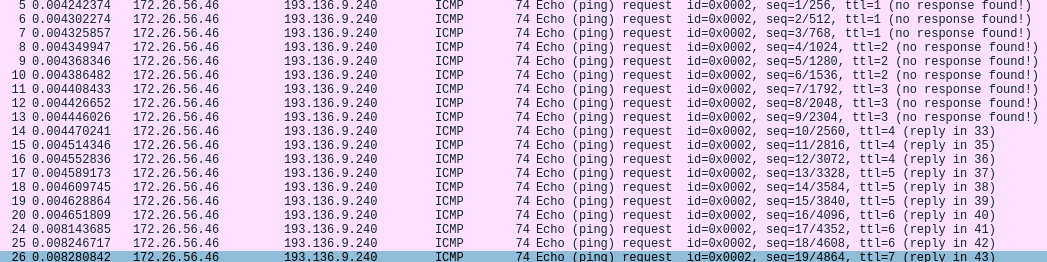
\includegraphics[width=500pt]{images/ParteI/Questao2/questao2-ICMPdaMaquina.png}
    \caption{Sequência de mensagens ICMP enviadas pela máquina.} \label{questao2-SequenciaICMP-1}
    \end{figure}

    \begin{minipage}{0.5\linewidth}
    \centering
        \begin{figure}[H]
        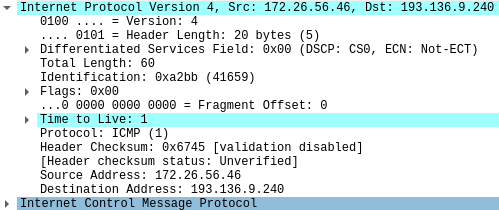
\includegraphics[width=0.95\linewidth]{images/ParteI/Questao2/questao2-PrimeiroPacoteCabecalho.png}
        \caption{Primeiro pacote com TTL=1.} \label{questao2-primeiroPacote}
        \end{figure}
    \end{minipage}
    \begin{minipage}{0.5\linewidth}
    \centering
        \begin{figure}[H]
        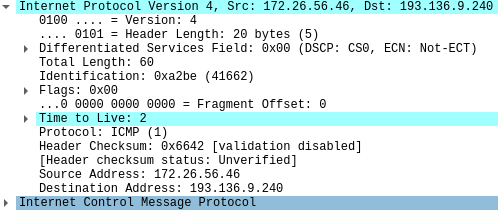
\includegraphics[width=0.95\linewidth]{images/ParteI/Questao2/questao2-primeiro2TTLCabecalho.png}
        \caption{Primeiro pacote com TTL=2.} \label{questao2-SegundoPacote}
        \end{figure}
    \end{minipage}

    \paragraph{}
    \paragraph{}
    \par Analisando os pacotes da sequência de mensagens ICMP enviadas pela máquina nativa, podemos inferir que alguns campos se alteram ao longo da sequência. Assim, conseguimos distinguir os seguintes campos: \textbf{\textit{Identification}, \textit{Checksum}} e \textbf{TTL}. O \textit{checksum} é um parâmetro de controlo de integridade do pacote, sendo, por isso, normal que o seu valor não coincida. Relativamente aos outros dois campos, é explicado na alínea seguinte.
    

\newpage
\subsubsection{Observa algum padrão nos valores do campo de Identificação do datagrama IP e TTL?}

    \par O campo de identificação é incrementado sequencialmente e o campo TTL vai incrementando em conjuntos de trẽs pacotes, ou seja, três pacotes são enviados com o mesmo valor (TTL = k) seguidos de outros três com o valor inteiro diretamente acima (TTL = k+1).
 

\subsubsection{Ordene o tráfego capturado por endereço destino e encontre a série de respostas ICMP TTL \textit{exceeded} enviadas ao seu computador. Qual é o valor do campo TTL? Esse valor permanece constante para todas as mensagens de resposta ICMP TTL \textit{exceeded} enviados ao seu \textit{host}? Porquê?}

    \begin{figure}[H]
    \centering
    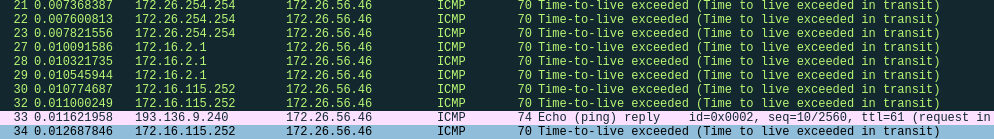
\includegraphics[width=500pt]{images/ParteI/Questao2/questao2-TTLExceeded.png}
    \caption{Sequência de mensagens ICMP enviadas pelo endereço destino.} \label{questao2-SequenciaICMP-2}
    \end{figure}
    
    \par O campo TTL não se mantém constante para todas as mensagens de resposta, tendo um valor diferente para cada \textit{host}. Isto acontece porque como os pacotes são enviados pelos \textit{routers} em que o TTL falha, o número de saltos necessários para atingir a nossa máquina ou definidos como \textit{default} pelos mesmos variam.
    
    
    
\newpage
% --------------------- QUESTÃO 3 ------------------------------
\subsection{Questão 3 - Fragmentação}

    \par De acordo com o requisito do enunciado, executamos o comando \textit{traceroute} definindo o tamanho do pacote para 4000 + 135 (nº do grupo) = \textbf{4135}.

    \begin{figure}[H]
    \centering
    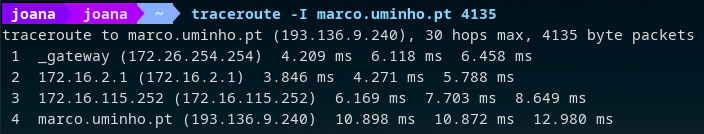
\includegraphics[width=400pt]{images/ParteI/Questao3/questao3-terminal.png}
    \caption{Resultado do comando \textit{traceroute} com tamanho de pacote definido.} \label{questao3-terminal}
    \end{figure}
    


\subsubsection{Localize a primeira mensagem ICMP. Porque é que houve necessidade de fragmentar o pacote inicial?}

    \begin{figure}[H]
    \centering
    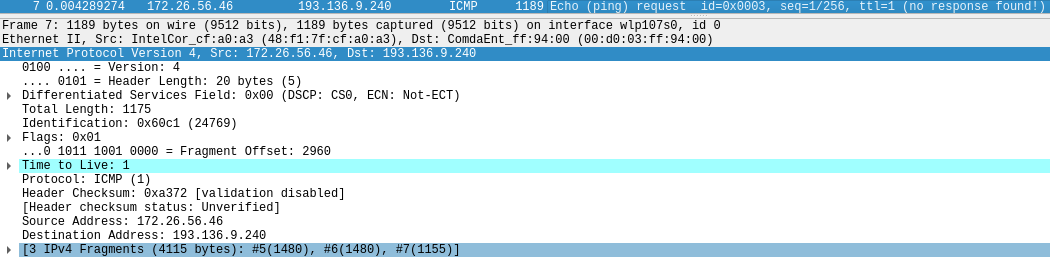
\includegraphics[width=500pt]{images/ParteI/Questao3/questao3-UltimoSegmento.png}
    \caption{Primeiro pacote ICMP enviado pela máquina.} \label{questao3-ICMP}
    \end{figure}
    
    \par Foi necessário fragmentar o primeiro pacote visto que o limite da camada de \textit{IP} é de 1500 \textit{bytes} em contraste com o tamanho do pacote a ser enviado (4135 \textit{bytes}), ou seja o MTU é inferior ao tamanho do pacote a ser enviado.

\subsubsection{Imprima o primeiro fragmento do datagrama IP segmentado. Que informação no cabeçalho indica que o datagrama foi fragmentado? Que informação no cabeçalho IP indica que se trata do primeiro fragmento? Qual é o tamanho deste datagrama IP?}

    \begin{figure}[H]
    \centering
    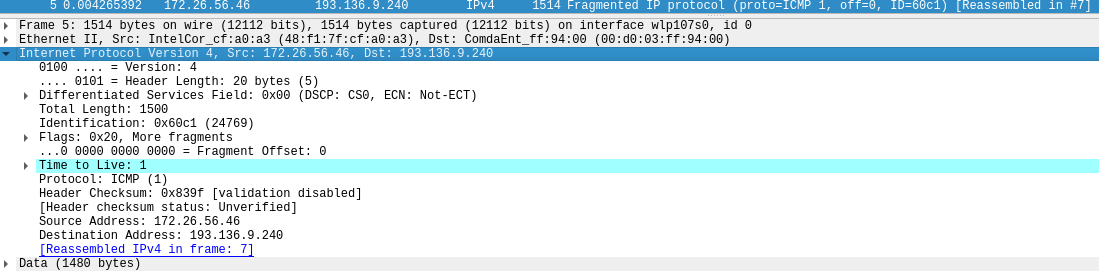
\includegraphics[width=500pt]{images/ParteI/Questao3/questao3-firstSegmentado.png}
    \caption{Primeiro pacote fragmentado.} \label{questao3-primeiroSeg}
    \end{figure}
    
    \par O cabeçalho indica-nos que o datagrama foi fragmentado pois tem a \textit{flag \textbf{More Fragments}} acionada. Para além disto, sabemos que se trata do primeiro fragmento do datagrama original pois o valor no campo \textit{\textbf{Fragment Offset}} é 0, ou seja, este datagrama tem um deslocamento de dados igual a 0 relativamente ao datagrama original. Assim, este datagrama tem um tamanho de 1500 \textit{bytes} (20 para cabeçalho e 1480 para dados).
    
    
\subsubsection{Imprima o segundo fragmento do datagrama IP original. Que informação do cabeçalho IP indica que não se trata do 1º fragmento? Há mais fragmentos? O que nos permite afirmar isso?}

    \begin{figure}[H]
    \centering
    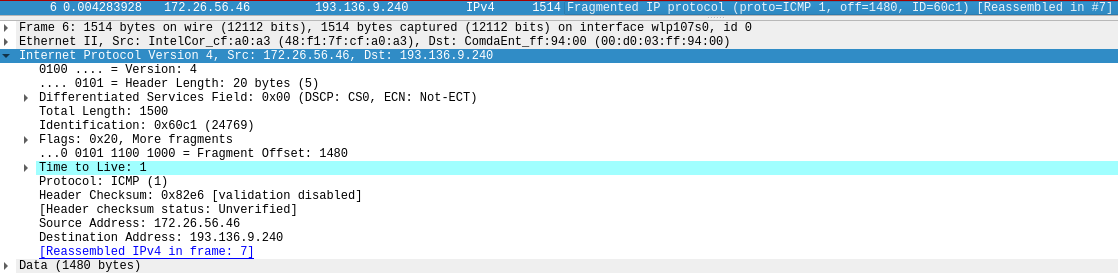
\includegraphics[width=500pt]{images/ParteI/Questao3/questao3-secondSegment.png}
    \caption{Segundo pacote fragmentado.} \label{questao3-segundoSeg}
    \end{figure}
    
    \par Conseguimos verificar, através do valor presente no campo \textit{\textbf{Fragment Offset}} do cabeçalho, que não se trata do primeiro fragmento do datagrama, uma vez que esse valor é diferente de 0, sendo, neste caso, 1480, indicando, por isso, um deslocamento de 1480 \textit{bytes} relativamente ao datagrama original. Para além disto, conseguimos denotar que se vão seguir mais fragmentos através do acionamento da \textit{flag \textbf{More Fragments}}.
    
\subsubsection{Quantos fragmentos foram criados a partir do datagrama original?}

    \par A partir do datagrama original, foram criados três fragmentos como podemos ver pelas Figuras acima. O primeiro fragmento (Figura \ref{questao3-primeiroSeg}) e o segundo (Figura \ref{questao3-segundoSeg}) com um total de 1480 \textit{bytes} de dados. Por fim, o último fragmento (Figura \ref{questao3-ICMP}) corresponde ao primeiro pacote ICMP enviado pela máquina, com um total de 1155 \textit{bytes} de dados.
    
    
\subsubsection{Indique, resumindo, os campos que mudam no cabeçalho IP entre os diferentes fragmentos, e explique a forma como essa informação permite reconstruir o datagrama original.}

    \par Os campos que se vão alterando ao longo da sequência de fragmentos são \textit{checksum}, \textit{flags}, \textit{offset} e o tamanho do último fragmento relativamente aos anteriores, uma vez que apenas este pode ter ou não o número máximo de dados por pacote. O valor de \textit{checksum}, como referido em alíneas anteriores, serve para verificar a integridade do pacote, no entanto, não tem relação direta com a reconstrução do datagrama original. Já os campos das \textit{flags} e o \textit{offset} permitem fazer a reconstrução do datagrama, na medida em que o \textit{offset} indica a posição do fragmento relativamente aos dados originais, permitindo a ordenação correta dos fragmentos, e as \textit{flags} permitem afirmar se estamos localizados no último pacote ou se ainda existem mais.
    
    
\subsubsection{Verifique o processo de fragmentação através de um processo de cálculo.}

    \begin{figure}[H]
    \centering
    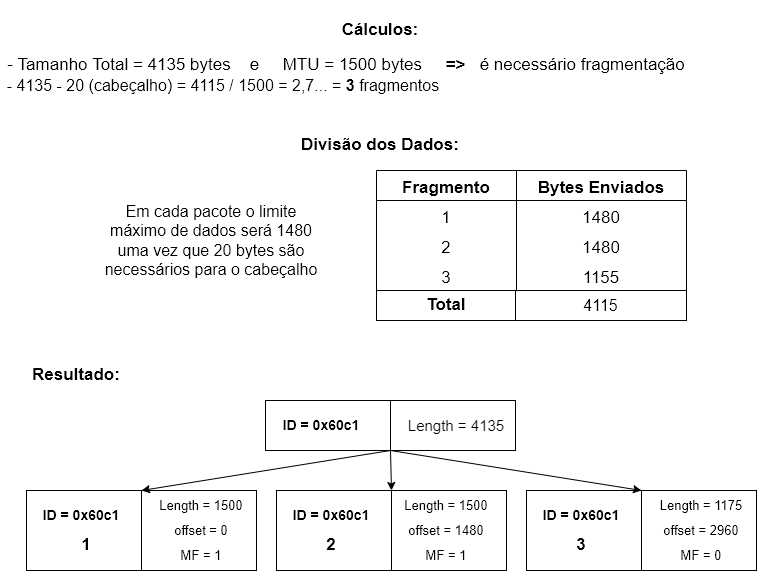
\includegraphics[width=490pt]{images/ParteI/Questao3/fragmentacao.png}
    \label{questao3-Calculo}
    \end{figure}
    
    \vspace{0.5cm}
    \par Como podemos verificar pelos cálculos, o datagrama original teria de ser dividido em três fragmentos. Os fragmentos mantêm o mesmo campo de identificação do datagrama original, alterando apenas as \textit{flags} de \textit{More Fragments} (MF) e o valor do \textit{offset} relativamente ao original. A \textit{flag} MF está apresentada com os valores 0 (equivalente ao valor '\textit{not set}') e 1, tendo estes o significado de não acionada e acionada, respetivamente.
    
    \par De forma adicional, podemos reparar que o \textit{overhead} de cabeçalho aumentou, uma vez que originalmente tínhamos apenas 20 \textit{bytes} de cabeçalho e devido à fragmentação obtivemos um conjunto de três cabeçalhos, ou seja, 60 \textit{bytes}.  
    Como consequência, houve um aumento do número total de \textit{bytes} transferidos na rede, pois no datagrama original seriam 4135 \textit{bytes} em contraste com a fragmentação, onde se registaram no total: 4115 (dados) + 3 * 20 (cabeçalho) = 4175 \textit{bytes}.
    
    \par Em suma, todos os valores calculados coincidiram com os valores presentes nos campos dos datagramas fragmentados capturados pelo programa.
    
    
\newpage
\subsubsection{Escreva uma expressão lógica que permita detetar o último fragmento correspondente ao datagrama original.}

    \par De acordo com os parâmetros do cabeçalho dos pacotes analisados nas alíneas acima, conseguimos deduzir os campos que afetam diretamente a deteção do último fragmento da \textit{stream}, sendo estes a \textit{flag more fragments} e o campo \textit{offset}. O valor do campo \textit{offset} tem de ser diferente de zero para assim concluirmos que, antes de mais, se trata de um datagrama fragmentado. A \textit{flag more fragments} transmite a informação se o fragmento se trata do último ou não. Por último, para o pacote fragmentado corresponder a um fragmento do original que procuramos, o campo de identificação tem de ser igual. Assim, apresentamos a expressão lógica capaz de detetar o último fragmento tendo em conta estes campos do cabeçalho:

    \paragraph{}
    \begin{minipage}{\linewidth}
        \centering
        \fbox{
        ID == original \space\space \&\& \space\space More Fragments == \textit{not set} \space\space \&\& \space\space offset \begin{math}  > 0 \end{math}
        }
    \end{minipage}
    
    \paragraph{}
    \par De seguida, de forma a testar a nossa expressão, executamos a mesma na secção de \textit{filter} da ferramenta \textit{Wireshark} com a única diferença de não incluirmos a verificação do campo de identificação, obtendo assim todos os últimos fragmentos de todos os datagramas que sofreram fragmentação. Como podemos conferir pela Figura \ref{questao3-ultima}, obtivemos o resultado esperado:
    
    \begin{figure}[H]
    \centering
    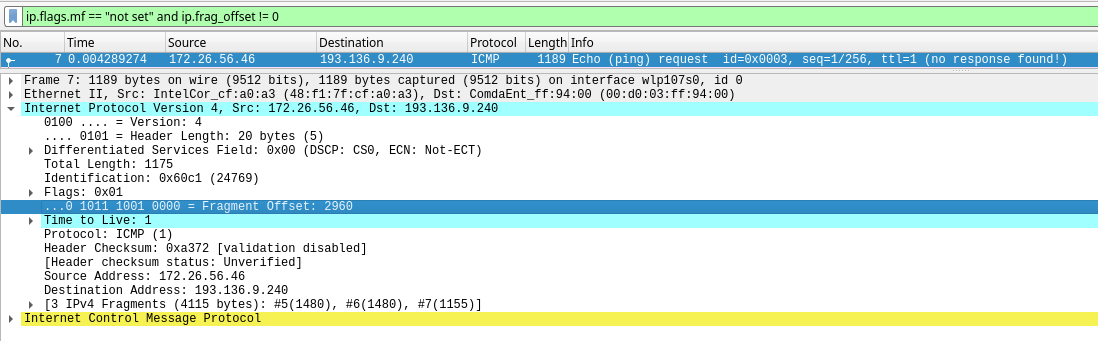
\includegraphics[width=490pt]{images/ParteI/Questao3/questao3-ultima.png}
    \caption{Verificação da expressão na ferramenta \textit{Wireshark}.}
    \label{questao3-ultima}
    \end{figure}